% TODO: Para cada modelo colocar como que é a entrada na forma de uma expressão matemática

\section{Tráfego}


\section{\acrfull{NN}}


\section{\acrfull{RNN}}

% RESOURCE: to explain recurrent neural networks (http://d2l.ai/chapter_recurrent-neural-networks/index.html)

% TODO: Falar que nem todos os dados são independentes, então a RNN serve para lembrar de alguns dados que já passaram pelo modelo para melhorar a performance.

% TODO: Falar que é melhor para predição aparentemente (pode ser algo a ver com o tipo de dados que temos)

% TODO: Falar que sofre de memória curta e outros defeitos

% TODO?: Falar que basicamente é um modelo feito para lidar com dados dependentes

\section{\acrfull{LSTM}}

\acrshort{LSTM} é utilizado para predição de tráfego e de informações que derivam de dados sequenciais/séries temporais, sendo possível encontrar diversos trabalhos na literatura que mostram sua eficiência quando comparado a outros métodos. Como descrito em \cite{Zainab_2018} e em \cite{Xiaolei_2015}, \acrshort{LSTM} é um tipo de \acrshort{RNN} que utiliza de estados anteriores e do estado atual da rede para gerar sua saída. Ao utilizar dos estados anteriores, a \acrshort{RNN} acaba por simular uma memória, melhorando sua capacidade de aprender. 

\begin{figure}[htb]
    \centering
    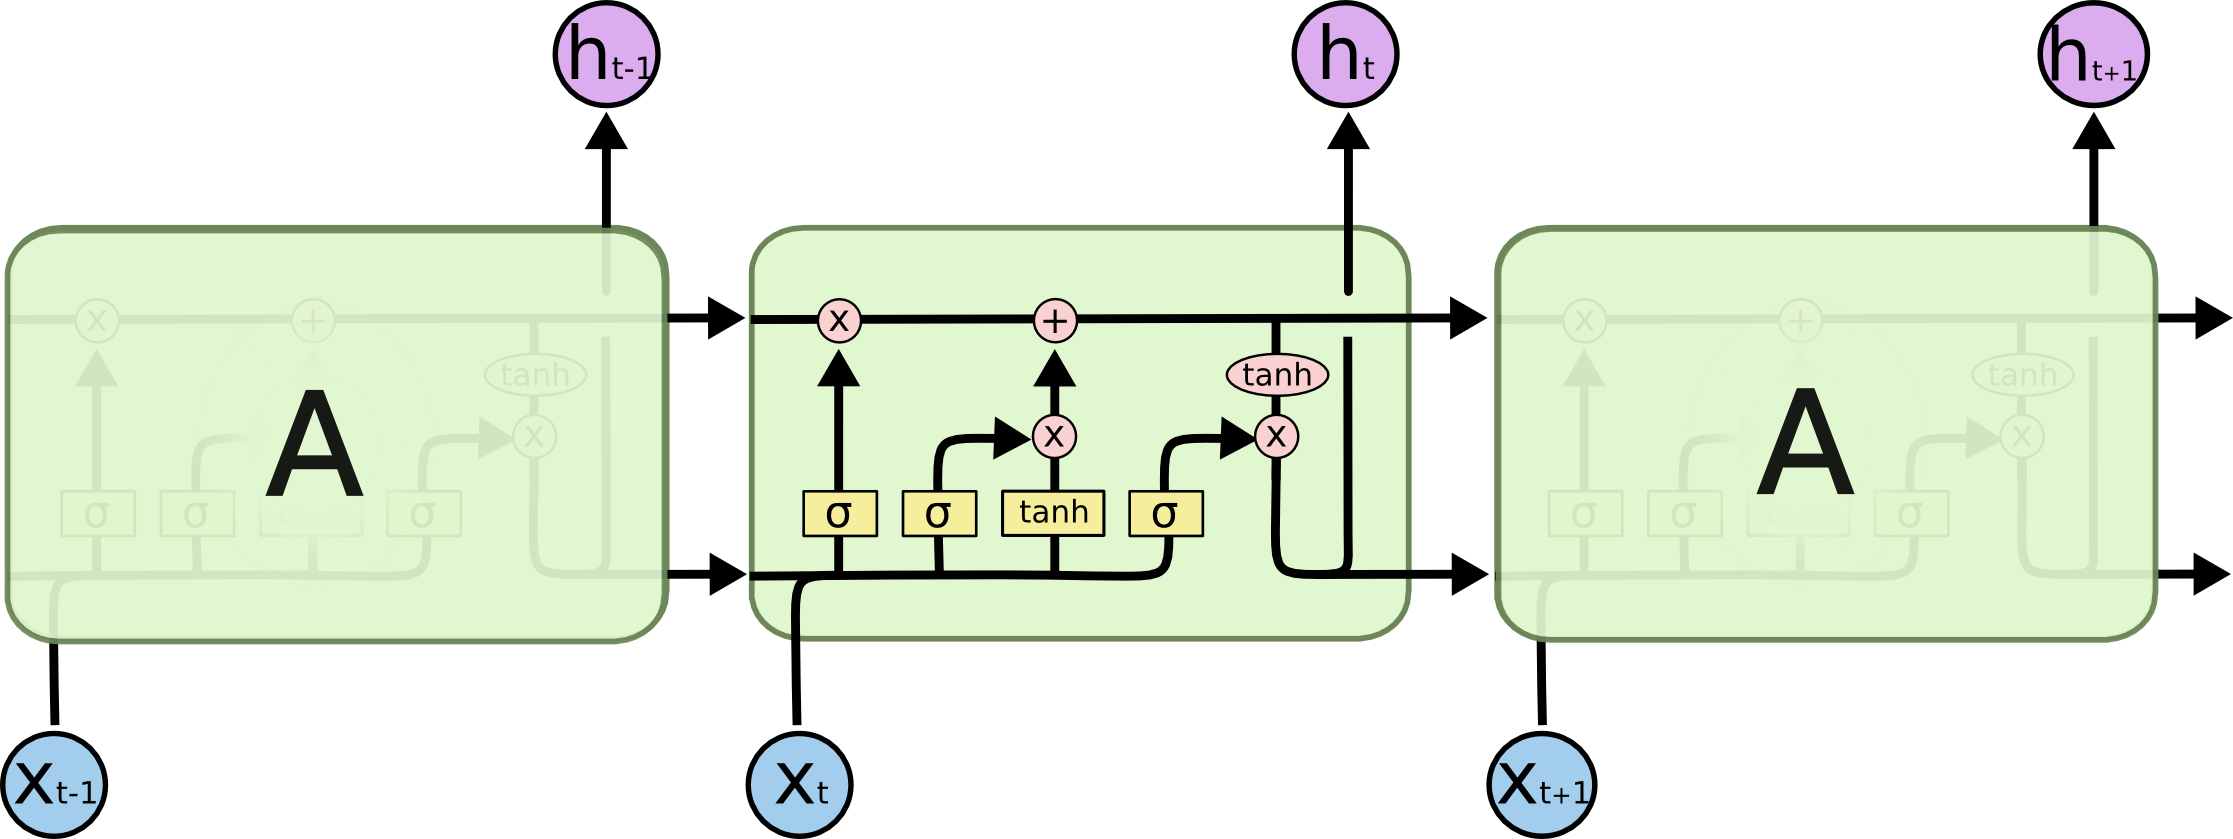
\includegraphics[scale=0.4]{lstm3.png}
    \label{figure:eixo}
    \caption[Representação de uma arquitetura LSTM]{Representação de uma arquitetura LSTM\footnotemark}
\end{figure}

\footnotetext{https://colah.github.io/posts/2015-08-Understanding-LSTMs/}

Porém, diferentemente de uma \acrshort{RNN}, o LSTM possui uma unidade a mais em seus blocos chamada de célula de memória. Esta célula é capaz de perceber as características mais latentes dos dados e descartar as menos importantes. Assim, o \acrshort{LSTM} consegue manter as características mais recorrentes na rede por mais tempo que uma \acrshort{RNN} comum. Por estes motivos, o \acrshort{LSTM} é excelente para modelar séries temporais e dados sequenciais.

Na célula de memória citada anteriormente, existem estruturas que são responsáveis pela característica de memória a longo prazo do \acrshort{LSTM}. A Porta de Entrada, a Porta do esquecimento e a Porta de Saída. Abaixo, explicaremos como cada um deles funciona:

\begin{itemize}
  \item Porta de Entrada: 
  
  \item Porta do Esquecimento: 
  \item Porta de Saída:
\end{itemize}

% TODO: Falar que podemos responder a quantidade de camadas da LSTM com o problema que RNN tem com back-propagation que o gradiente começa a diminuir exponencialmente. Mas tem que dar uma conferida melhor.

\section{\acrfull{GRU}}

\section{\acrfull{RF}}

% TODO: adicionar o criador

% TODO: ler o artigo do criador ou usar o artigo de alguém que tenha explicado  random forest

% TODO: rf usa o bagging com decision tree

% The random forest combines hundreds or thousands of decision trees, trains each one on a slightly different set of the observations, splitting nodes in each tree considering a limited number of the features. The final predictions of the random forest are made by averaging the predictions of each individual tree.

% TODO: explicar o motivo da random forest não over-fitar tanto

\textit{\acrshort{RF}} é um método de aprendizagem de máquina muito utilizado para classificação e regressão. O método é utiliza do \textit{Bagging} (\textit{\textbf{B}ootstrap \textbf{Agg}regation}) coma árvores de decisão, para evitar sobre-ajuste. Para isso, ele modifica o algoritmo de criação das árvores de decisão limitando a quantidade de características (\textit{features}) do conjunto de dados que vai ser utilizado. É comum implementações limitarem a quantidade de características (\textit{q}) para $ \sqrt{q} $ ou $ \frac{q}{3} $.

\subsection{Bagging}



\subsection{Árvores de Decisão}

Segundo \citet{}

 Árvores de decisão sobre-ajustam muito fácil no conjunto de dados por ser muito flexível e poderoso, memorizando parte do conjunto de dados. Podendo, por exemplo, criar uma árvore que cada folha corresponde a somente um elemento.

% https://towardsdatascience.com/an-implementation-and-explanation-of-the-random-forest-in-python-77bf308a9b76
 Algoritmos podem ser flexíveis e correr risco de sobre-ajuste ou ser inflexíveis e não conseguir se ajustar nos dados. Modelos flexiveis demais podem  meomorizar os dados e modelos inflexiveis presupõe informações sobre os dados.
 Árvore de decisão é flexível se não for limitar o tamanho da árvore e inflexível se vc limitar demais o tamanho da árvore. Isso é chamado de bias-variance tradeoff.

\subsubsection{Impureza de Gini}

\subsection{\textit{\acrshort{RF}}}


\section{\acrfull{SVM}}

% RESOURCE: to learn better how random forest work (https://stackabuse.com/random-forest-algorithm-with-python-and-scikit-learn/)

